\chapter{Trees} \label{tree}

\subsection{Balancing Trees}

A tree is balanced when each level of the tree (except possibly the last
level) has as many nodes as it can hold. The tree below is balanced
because all of the nodes have both left and right subtrees except for
the ones on the last level.

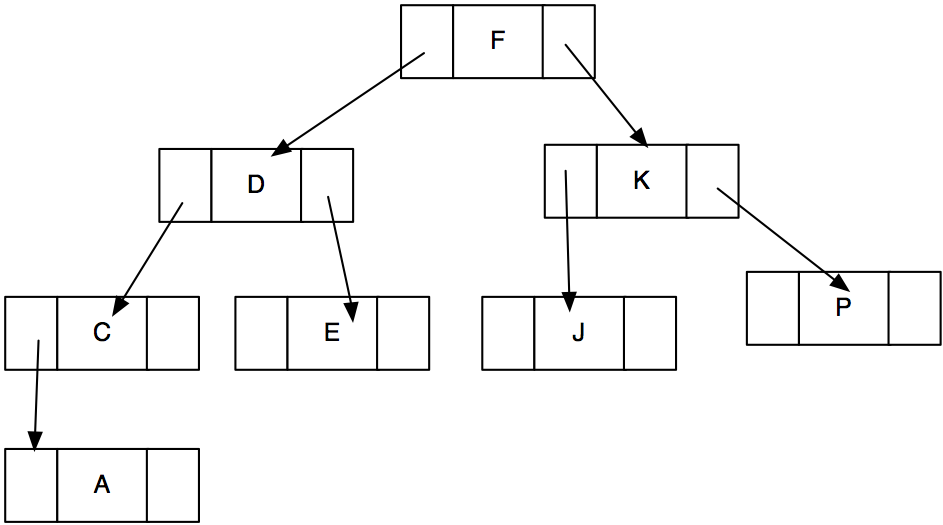
\includegraphics[width=6.00000in]{pictures/image6.pdf}

Because trees can be very sensitive to input order, they can quickly
become unbalanced.  For example,  try to sketch the tree that results from adding the
following nodes (in the order given): A C D E F J K P    

A tree can be rebalanced , but the rebalancing operation must not change
the order of the nodes in the tree and it must be more efficient than
simply rebuilding the tree by randomizing the input order. The operation
used to rebalance a tree is a rotation.

The figure below shows an unbalanced tree. The tree is unbalanced to the
right because the right subtree is higher than the left subtree.  The tree can be rebalanced by rotating the tree to the right. The
rotation operation can only work if the middle node (the one that will
be the new root) has no left tree.

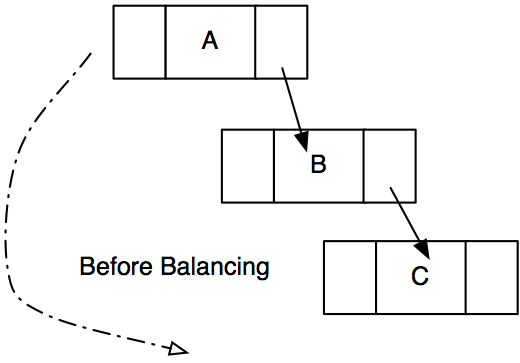
\includegraphics[width=3.47222in]{pictures/image7.pdf}

After the rotation the tree would look like this.

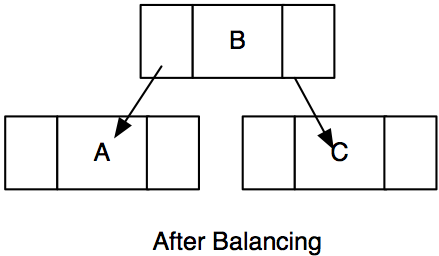
\includegraphics[width=2.93056in,height=1.29167in]{pictures/image8.pdf}

A tree that is unbalanced to the left can be fixed using a rotation to
the right. A right rotation is only possible if the middle node has no
right branch.

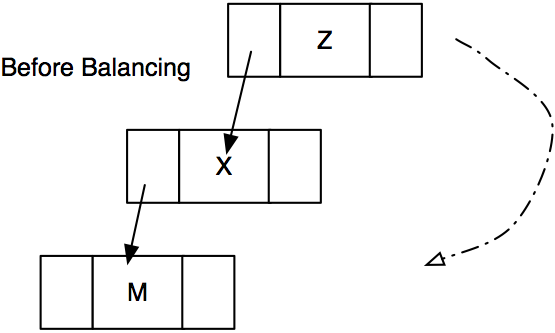
\includegraphics[width=3.47222in]{pictures/image9.pdf}

After the rotation, the tree looks like this:

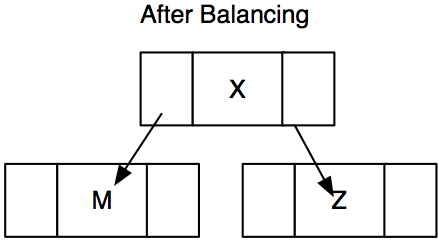
\includegraphics[width=2.93056in]{pictures/image10.pdf}

A series of rotations can be used to balance a large unbalanced tree. In the next two chapters we will explore the use of rotations to
 balance binary trees and search trees.



\section{Binary Search Trees}

One common application for binary trees is to use them as a search tree for quickly finding stored information. Binary trees are fast, as long as they are balanced. Unfortunately, in the worst case scenario (if the data is entered sorted, for example), a binary search tree has O(N) complexity for insertion and retrieval. Why is this?

%Using the applet found at:\href{http://people.ksp.sk/%7Ekuko/bak/}{ http://people.ksp.sk/\textasciitildekuko/bak/}, create a binary search tree (BST) by inserting the numbers between 1 and 9 into the tree, in order. What do you notice about the tree? (unclick the pause button once you understand what the insertion is doing)

Clear the tree and insert the same numbers in the following order 5 3 7 4 2 8 6 9 1 . What do you notice about the tree this time?

To mitigate the problems associated with the order of operations, specialized binary search trees have been developed that maintain the balance of the tree as data is entered and removed. There are many types of search trees including AVL trees, B trees, 2-3 trees, Red-black trees, Splay trees, skip lists and heaps. We will examine two in this class, AVL trees and B trees.

After working through this material, check your understanding of search trees by doing the practice quiz.

\section{AVL trees}

The AVL tree was proposed in 1962 as a solution to the problems with binary search trees. It is named in honour of the authors of the original paper introducing the tree, Adel'son-Velskii and Landis.

An AVL tree maintains the balance of the binary tree by rearranging the tree on insert and delete to carefully manage the height difference of the children of every node.

For example, in the three shown below 5 has just been inserted into the tree. The left subtree of node 82 has height of 2 and the right subtree of node 82 has height of 0. The height difference between the two subtrees of node 82 is greater than one, which indicates that the tree must be rebalanced.

\begin{figure}[H]
\centering
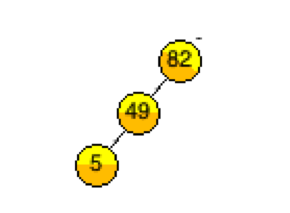
\includegraphics{pictures/tree1.png}
\caption{Unbalanced Tree}
\label{fig:tree1}
\end{figure}

A right rotation is performed on the left child and the rebalanced tree looks like the one below. Notice that the root node of the tree has changed (it is now node 49) but the tree still meets the requirements for a binary tree.

\begin{figure}[H]
\centering
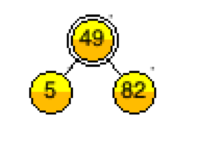
\includegraphics{pictures/tree2.png}
\caption{Rebalanced Tree}
\label{fig:tree2}
\end{figure}

Node 74 is then added to the tree. After insertion the right subtree of node 49 has a height of two and the left subtree has a height of one. The difference between the two subtrees is one which indicates that the tree does not need to be rebalanced.

\begin{figure}[H]
\centering
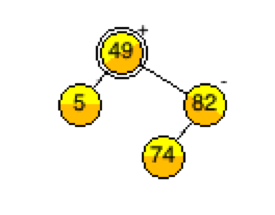
\includegraphics{pictures/tree3.png}
\caption{74 addition. Still balanced}
\label{fig:tree3}
\end{figure}

After inserting both 41 and 38 the tree is again unbalanced. While the height difference between the subtrees of node 49 is only one, the left subtree of node 5 has a height of zero and the right subtree has a height of two, which indicates a need to rebalance the tree.

\begin{figure}[H]
\centering
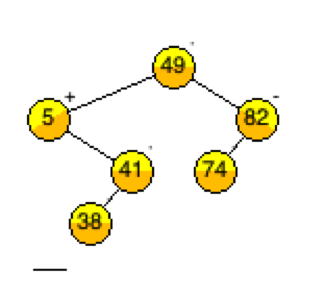
\includegraphics{pictures/tree4.png}
\caption{41 and 38 added. Tree is now unbalanced}
\label{fig:tree4}
\end{figure}

The tree must be rebalanced in two steps. Ultimately we must replace node 5 with node 38 and make node 5 a child of node 38. The first step to rebalancing this tree is to do a right rotation with node 5's right child which switches the places of nodes 38 and 41. Nodes 5, 38, and 41 are now in order (and all in right subtrees).

\begin{figure}[H]
\centering
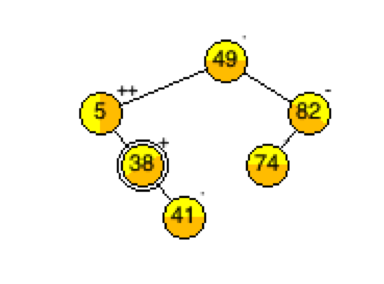
\includegraphics{pictures/tree5.png}
\caption{First rotation}
\label{fig:tree5}
\end{figure}

The second step is to do a left rotation with node 5, which rotates node 38 into the parent position.

\begin{figure}[H]
\centering
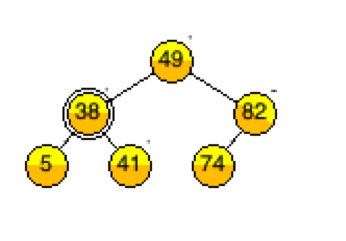
\includegraphics{pictures/tree6.png}
\caption{Second rotation}
\label{fig:tree6}
\end{figure}

After adding 21, then 25 to this tree, the left subtree of 38 is unbalanced.

\begin{figure}[H]
\centering
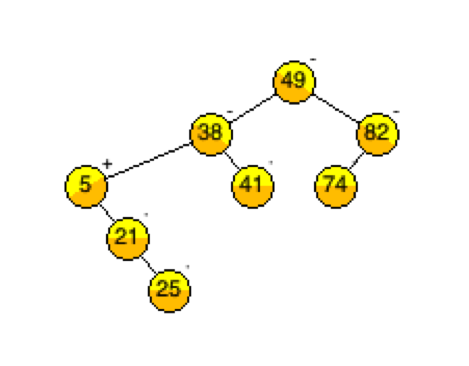
\includegraphics{pictures/tree7.png}
\caption{21 addition. Tree is now unbalanced}
\label{fig:tree7}
\end{figure}

The tree can be rebalanced by doing a left rotation on the left subtree of 38 (the one rooted at 5).

\begin{figure}[H]
\centering
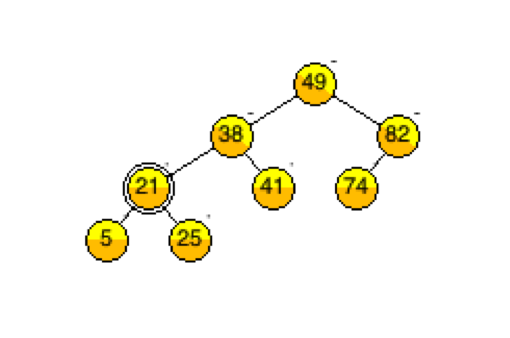
\includegraphics{pictures/tree8.png}
\caption{Left rotation on 5}
\label{fig:tree8}
\end{figure}

If 35 is added to this tree, node 21 is still balanced, but node 38 is out of balance.

\begin{figure}[H]
\centering
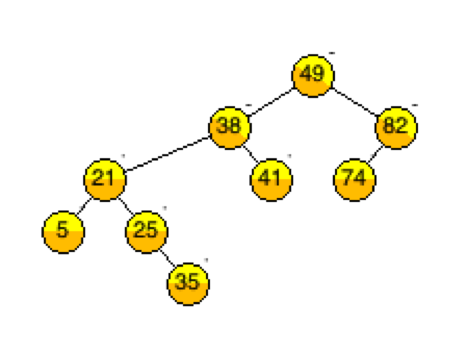
\includegraphics{pictures/tree9.png}
\caption{35 addition. Tree is now unbalanced}
\label{fig:tree9}
\end{figure}

Two rotations are required to rebalance the resulting tree. First the left subtree of node 38 must be rotated and then the entire subtree tree rooted at 38 must be rotated. There is often a need for more than one rotation to maintain balance over the entire AVL tree.


\begin{figure}[H]
\centering
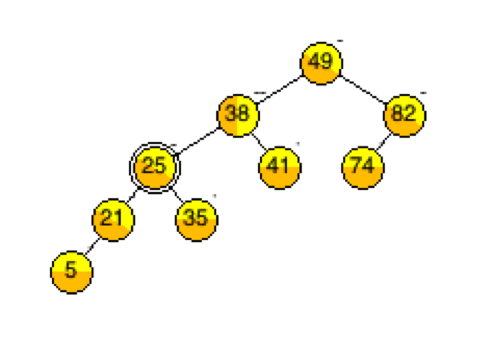
\includegraphics{pictures/tree11.png}
\caption{First rotation. Right rotation on 38 next.}
\label{fig:tree11}
\end{figure}

The same rotation rules apply when deleting nodes from the tree. While the rotations can seem complicated, the AVL tree is actually fairly simple once you understand the patterns for selecting the rotations.

To facilitate the balancing of the trees, each node in an AVL tree contains an additional member that is the height of the subtree rooted at that node. It is simpler to count a tree of one node as height 1 for AVL trees than to start counting at zero.

\begin{figure}[H]
\centering
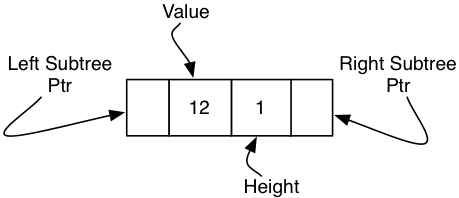
\includegraphics{pictures/tree12.png}
\caption{Tree node}
\label{fig:tree12}
\end{figure}

A balanced AVL tree has no subtrees for which differences in height between left and right children is more than 1.

Consider the example below: The root node in the first tree has a height of 2 because it has a left child. The child has a height of 1.

\begin{figure}[H]
\centering
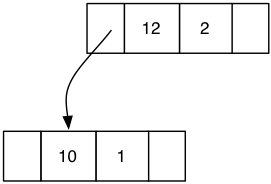
\includegraphics{pictures/tree13.png}
\caption{Tree node with 10 left child}
\label{fig:tree13}
\end{figure}

The next example shows a tree of height 3, with the heights of the children shown as well. Notice that the root node has two children, one with a height of 2 and one with a height of 1. Because the difference in heights of these two children is 1, the tree is still a balanced AVL tree.

\begin{figure}[H]
\centering
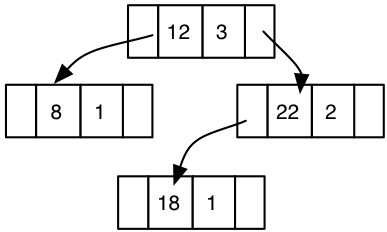
\includegraphics{pictures/tree14.png}
\caption{Balanced Tree}
\label{fig:tree14}
\end{figure}

While the examples in the picture show an AVL tree storing integers, it is far more useful to have an AVL tree that stores void pointers in much the same way as the binary tree does (from the previous lesson). One design for the structs for an AVL tree is shown below. Notice that the AVLTree is separate from the AVLTreeNodes. This permits the use of function pointers to compare and destroy the void data types without any requirement that the tree library has knowledge of what those data types are. It also means the the
\begin{verbatim}
struct  AVLTreeNode{
    TreeDataTypePtr data;
    int nodeBalance;
    struct AVLTreeNode * left;
    struct AVLTreeNode * right;
};\end{verbatim}
\begin{verbatim}
struct AVLTree {
    struct AVLTreeNode * root;
    int (*compare) (TreeDataTypePtr data1, TreeDataTypePtr data2);
    void (* destroy) (TreeDataTypePtr data);
};\end{verbatim}

The interface/function requirements for an AVL tree are the same as those of any binary tree. The user of the AVL tree library will need at least the following functions (function names are unimportant, it's the functionality that is important).
\begin{verbatim}
Tree * createAVLTree(int (*comparePointer) (TreeDataTypePtr data1, TreeDataTypePtr data2), void (*destroyPointer) (TreeDataTypePtr));
void  destroyAVLTree(Tree * toDie);
void addToTree(Tree * theTree, TreeDataTypePtr data);
void removeFromTree(Tree * theTree, TreeDataTypePtr data);
bool isInTree(Tree * theTree, TreeDataTypePtr data);\end{verbatim}

Additionally, the tree ADT will be more useful with the inclusion of pre/post and in order iterators. A simple way to implement iterator functionality is to permit only one iterator at a time on any given tree and to require a flag as a parameter to the iterator function to indicate the desired traversal. The functions required for such an iterator include a function to initialize the iterator and one to get the next value from the iterator.
\begin{verbatim}
void  initializeIterator(Tree * theTree, int traversalType);
TreeDataTypePtr interatorNext(Tree *theTree);\end{verbatim}

Finally, the user of the tree ADT might appreciate some utility functions to help with writing specialized operations for the tree. These might include functions for determining if the tree is empty and functions for examining subtrees of the tree.
\begin{verbatim}
bool isTreeEmpty(Tree * theTree);
Tree * getLeftSubtree (Tree *);
Tree * getRightSubtree (Tree *);
TreeDataTypePtr getRootData(Tree *);\end{verbatim}

The functions listed above comprise the programming interface that a \textbf{user} of the ADT would interact with. The AVL tree needs several functions that are used only by the internal operations of the tree itself. In particular, all of the programming interface functions have a parallel internal function that operates recursively on the nodes of the tree. Those functions are joined by the functions to perform the required rotations to keep the tree balanced. In the prototypes below COMPAREPTR and DESTROYPTR are the function pointers to the compare and destroy functions.
\begin{verbatim}
TreeNode * insert(TreeNode * root, TreeDataTypePtr data, COMPAREPTR);
TreeNode * delete(TreeNode * root, TreeDataTypePtr data,COMPAREPTR, DESTROYPTR);
TreeNode * find(TreeNode * root, TreeDataTypePtr data, COMPAREPTR);
TreeNode * findMin(TreeNode *);
TreeNode * findMax(TreeNode *);
bool isEmpty(TreeNode * root);
void destroy(TreeNode * root,DESTROYPTR);
  \end{verbatim}
 
\subsection{Balancing AVL Trees}
Most AVL tree functions are nearly identical to the functions found in a Binary Tree ADT with the exception of the insert and delete functions. Insert and delete have an additional balancing step that is invoked to ensure that the AVL tree remains in a balanced state after each insertion and deletion. An AVL tree is said to be balanced when the height difference between left and right subtrees is either 0 or 1 for every node in the tree. Some implementations keep track of the height of a node (from leaf to current node, starting counting at 1), some implementations keep track of the positive or negative balance factor for each node. We will use the heights of nodes to calculate the balance factor at run time.

When a tree becomes unbalanced, there are four possible situations:
\begin{itemize}
	\item a) the imbalance occurs in right subtrees
	\item b) the imbalance occurs in left subtrees
	\item c) the imbalance occurs in a right then left subtree
	\item d) the imbalance occurs in a left then right subtree
\end{itemize}



Each of the images below shows a three node tree that matches each of the cases above. Notice that each root node has a height of 3, has a single child that is height two, which means that the difference in heights of the nodes right and left children is greater than one.

\begin{figure}[H]
\centering
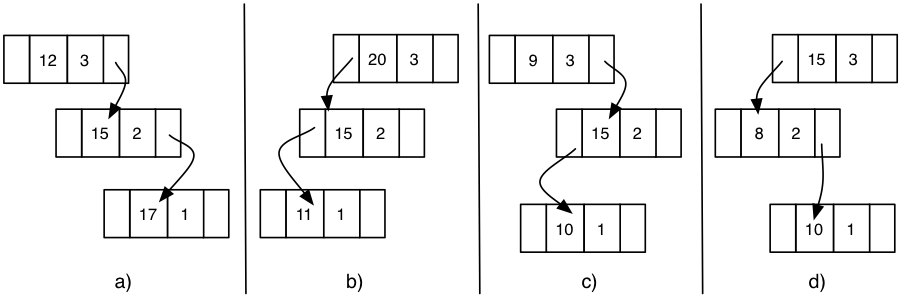
\includegraphics{pictures/tree15.png}
\caption{Unbalanced Tree Cases}
\label{fig:tree15}
\end{figure}

The solution to such imbalances is to rotate the subtree to restore balance. In all cases it is important to keep the ordering of the binary tree intact.

These cases hold even if the tree is a complete tree in which all nodes have children. The children of the newly assigned root in rotated subtrees are reassigned to the new children, maintaining the binary tree ordering.

Lets look at them case by case.\newline

\textbf{Case A: Imbalance to the right -$>$ Left Rotation.}

\begin{figure}[H]
\centering
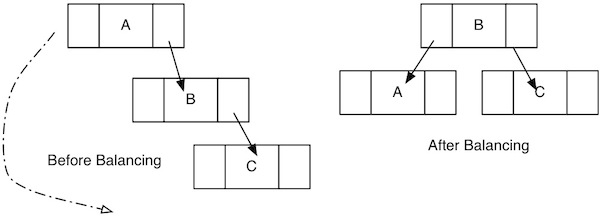
\includegraphics[width=0.5\textwidth]{pictures/leftrotate.jpg}
\caption{Left Rotation}
\label{fig:leftrotate}
\end{figure}

\begin{figure}[H]
\centering
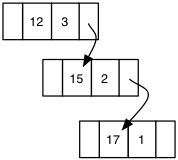
\includegraphics{pictures/tree16.png}
\caption{Right Imbalance}
\label{fig:tree16}
\end{figure}

Node 12 violates the AVL property because its right subtree has height two and its left subtree has height zero.

In this case, we know that node 12’s child (15) has a value that is between node 12 and the grandchild (17). We know this because the tree is a binary tree and these are all right children.

We can make 15 the new root of this subtree, make 12 its left child, and restore balance to the tree.

This is called a Single rotation. The resulting subtree is shown below with the heights updated. Note that 15 is now of height 2 and 12 and 17 each have height of 1.

Any left child of node 15 will become the right child of node 12 after the rotation. This is always possible because node 12 had node 15 as the right child initially and the pointers are simply swapped.

\begin{figure}[H]
\centering
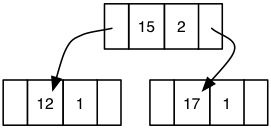
\includegraphics{pictures/tree17.png}
\caption{Balanced Tree}
\label{fig:tree17}
\end{figure}


\textbf{Case B: Imbalance to the left -$>$ Right rotation}

\begin{figure}[H]
\centering
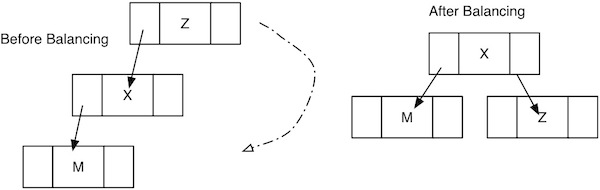
\includegraphics[width=0.5\textwidth]{pictures/rightrotate.jpg}
\caption{Right Rotation}
\label{fig:rightrotate}
\end{figure}
\begin{figure}[H]
\centering
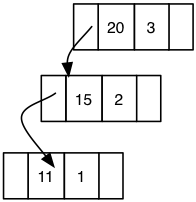
\includegraphics{pictures/tree18.png}
\caption{Left Imbalance}
\label{fig:tree18}
\end{figure}
\begin{itemize}
	\item This case is the mirror image of Case A.
	\item Node 20 is violating the AVL property. We know that its left child has a value that is ‘between’ node 20 and its grandchild.
	\item Node 15 becomes the new root, Node 20 becomes the right child and node 11 remains as the left child.
	\item This is also a single rotation (to the right).
\begin{itemize}
	\item Any right child of node 15 becomes the left child of node 20 after the rotation.
\end{itemize}
\end{itemize}

\textbf{Case C: Imbalance in left subtree of right child – double rotation}

\begin{figure}[H]
\centering
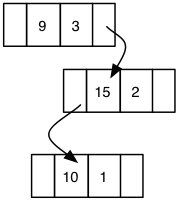
\includegraphics{pictures/tree19.png}
\caption{Imbalance in left subtree of right child}
\label{fig:tree19}
\end{figure}

\begin{itemize}
	\item In this case, a single rotation will not fix the balance problem. Because 10 is the value that is in the middle of 9 and 15, a simple rotation selecting 15 as the new root does not work.
	\item Instead we perform two rotations. The first is a right rotation on the child of the imbalanced node. This rotation has the effect of making node 10 a child of node 9 and making node 15 a child of node 10.
\begin{itemize}
	\item Any right child of node 10 becomes the left child of node 15
\end{itemize}
	\item The second rotation is a left rotation on the imbalanced node, which will restore balance to the tree.
\begin{itemize}
	\item Any left child of node 10 becomes the right child of node 9
\end{itemize}
\end{itemize}

\begin{figure}[H]
\centering
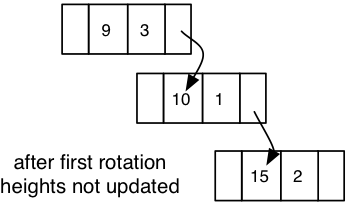
\includegraphics{pictures/tree20.png}
\caption{After first rotation. Right imbalance}
\label{fig:tree20}
\end{figure}

\begin{figure}[H]
\centering
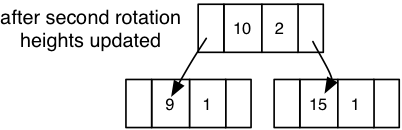
\includegraphics{pictures/tree21.png}
\caption{Balanced Tree}
\label{fig:tree21}
\end{figure}



\textbf{Case D: Imbalance due to right child of left subtree -$>$ double rotation}

\begin{figure}[H]
\centering
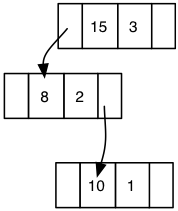
\includegraphics{pictures/tree22.png}
\caption{Imbalance in right subtree of left child}
\label{fig:tree22}
\end{figure}
\begin{itemize}
	\item This case is a mirror image of Case 3. You begin by doing a left rotation on the left child of the imbalanced node.
\begin{itemize}
	\item The left child of node 10 becomes the right child of node 8
\end{itemize}
	\item The balancing is finished by doing a right rotation on the imbalanced node.
\begin{itemize}
	\item The right child of node 10 becomes a left child of node 15
\end{itemize}
	\item In this case the result is a tree rooted at 8.
\end{itemize}



\subsection{AVL Tree Pseudocode}

An AVL tree ADT needs to be able to find the height of the node, it needs functions to rotateRight (with left child) and to rotateLeft (with right child). The insert function for an AVL tree can be easily written as a recursive function. An iterative function can be written to be slightly more efficient, but is much harder to write and debug (and to read).

The pseudocode is given for insert and for one set of rotations. The remaining two rotation algorithms are mirror images of the two given. Delete is somewhat more complicated for an AVL tree. Often a lazy delete is implemented where elements are simply marked as deleted and not actually removed from the tree. This is an effective strategy if elements are not deleted often or if there are duplicate elements in the tree.
\begin{verbatim}
insert(TreeNode * treeRoot, DataType * data): TreeNode *

  if treeRoot == NULL  create a new node with the data, return node
  else
    if the data is less that the treeRoot
      treeRoot->left = insert (treeRoot->left, data)
      if (height of treeRoot left child is more than 1 bigger than height of right child)
        if (data is less than the left child)
          treeRoot = rotateRightWithLeftChild(treeRoot)
        else
          treeRoot=doubleRotateWithLeftChild(treeRoot)
          
    else if the data is bigger than the treeRoot data
      treeRoot->right = insert(treeRoot->right, data)
      if (height of treeRoot right child is more than one taller than height of left child)
        if (data is greater than element of right child)
          treeRoot = rotateLeftWithRightChild(treeRoot)
        else
          treeRoot = doubleRotateWithRightChild(treeRoot)
          
  treeRoot->height = max of child heights +1
  return treeRoot
\\

rotateRightWithLeftChild(TreeNode * oldRoot): TreeNode *
  TreeNode * temp = oldRoot->left
  oldRoot->left = temp->right
  temp->right = oldRoot
  temp->height = max of children's heights +1
  oldRoot->height = max of children's heights +1
  return(temp)
\\

doubleRotateWithLeftChild (TreeNode * oldRoot): TreeNode *
  oldRoot->left = rotateWithRightChild(oldRoot->left)
  oldRoot = rotateWithLeftChild(oldRoot)
  return(oldRoot)
\\ 	
\end{verbatim}
\newpage
\section{B-Trees}

Suppose that you have so much data to manage that the resulting data structure cannot be held in the memory of the computer. In this case, the data structure and data must reside on persistent storage (usually a disk), which dramatically changes the cost of some operations. It is far more expensive in terms of time and complexity to read/write information on a disk than it is from computer memory. One disk access takes at least 100 000 times longer than a single operation in memory, so a disk-based ADT must be designed to minimize the number of disk accesses.

Even with a perfectly balanced AVL tree, the number of disk accesses to access information will be O(log n). Suppose the data set in question has one million entries, log2 of one million is approximately 20. If we guess that a hard drive has a seek time of 15 milliseconds, the optimistic time for a disk-based AVL tree is about 1/3 of a second per operation. That is far too slow for any type of modern data management system.

B-Trees are a data structure that is design to reduce the number of disk accesses to a small constant number. The algorithms for operations are a bit more complicated than for other trees, but the result is a search tree that minimizes disk accesses.

B-Trees are based on the idea of adding more branches to the tree, creating an m-ary search tree rather than a binary search tree.

\begin{figure}[H]
\centering
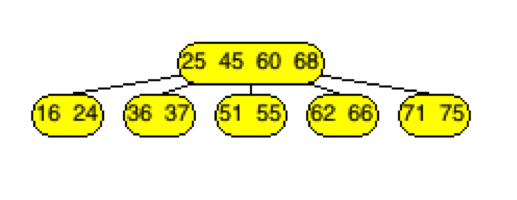
\includegraphics{pictures/tree23.png}
\caption{B-Tree}
\label{fig:tree23}
\end{figure}

The image above shows a small b-tree with a single root node and five children. Notice how each node in the b-tree holds more than one value. There are many specialized versions of b-trees. We are looking only at the general case.
\begin{itemize}
	\item A b-tree is an m-ary tree where M is the maximum number of children. It
	\item Each node in a b-tree contains up to m-1 keys
	\item The nodes in a b-tree are larger than many nodes in other trees. It is more efficient to read a large amount of data once from a disk than it is to read several small amounts of data.
	\item The keys in each node are stored in ascending order.
	\item Each key in a node is the root of a subtree that contains keys that are less than or equal to that key, but greater than any preceding key.
	\item Each node in the b-tree also contains a rightmost subtree that contains all the keys that are larger than the last key in the node.
	\item B-tree nodes do not always have the same number of children as the other nodes in a tree. However, there is a minimum number of children that each node must have that is set for each tree. Usually the minimum number of children is approximately half of the maximum number of children.
	\item All of the leaves in a b-tree are at the same depth
	\item The height of a b-tree is approximately logm N where m is the maximum number of children that a node can have.
\end{itemize}

The size of the nodes is managed by splitting and combining nodes during insert and delete operations. For example, the image below shows a b-tree with 5 keys. The maximum number of children allowable for this tree s 6 (one for each key and one for the right-most position). On the next insertion the node must be split.

\begin{figure}[H]
\centering
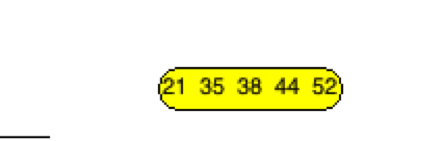
\includegraphics{pictures/tree24.png}
\caption{Balanced B-Tree}
\label{fig:tree24}
\end{figure}

35 is inserted into the tree, and the result is a tree that has two levels and three nodes. Notice that the root node has violated the minimum number of children rule, but that the child nodes have at least the minimum number of children (4 and 3). Sometimes it is necessary for the root node to have fewer children.

\begin{figure}[H]
\centering
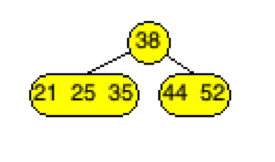
\includegraphics{pictures/tree25.png}
\caption{Split B-Tree}
\label{fig:tree25}
\end{figure}

After a few more insertions, the b-tree has a right most node that is nearly full.

\begin{figure}[H]
\centering
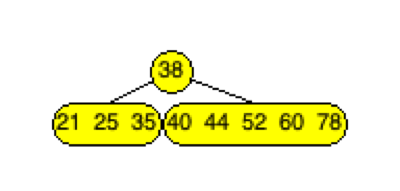
\includegraphics{pictures/tree26.png}
\caption{Full right node}
\label{fig:tree26}
\end{figure}

The insertion of 65 into this tree results in an overfull node that must be split.

\begin{figure}[H]
\centering
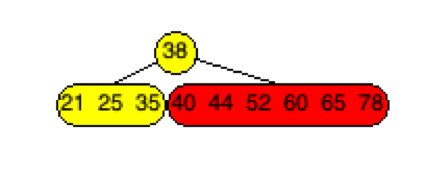
\includegraphics{pictures/tree27.png}
\caption{Over-full right node}
\label{fig:tree27}
\end{figure}

Since the root node has too few children, the node is split into a subtree rooted at the middle value, and then the middle value is combined with the root node to make a larger node.

\begin{figure}[H]
\centering
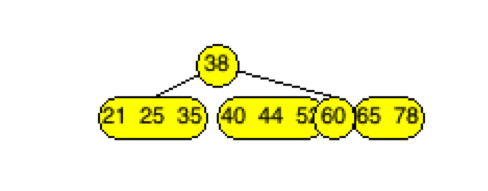
\includegraphics{pictures/tree28.png}
\caption{Splitting of right node}
\label{fig:tree28}
\end{figure}

\begin{figure}[H]
\centering
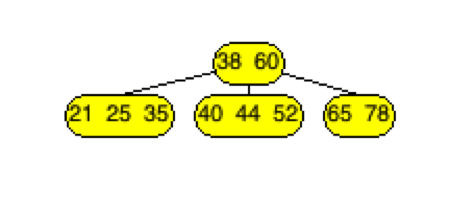
\includegraphics{pictures/tree29.png}
\caption{Split right node, 60 combined with parent node}
\label{fig:tree29}
\end{figure}

If a key is deleted from a node, leaving too few children in the node, a key is removed from a sibling to add to the too-empty node. This process often involves adding a new key to the parent, and moving a key from the parent into the too-empty child. Below is a picture showing the effect of removing key 78 from the tree shown above. In the first picture, node 65 is too empty.

\begin{figure}[H]
\centering
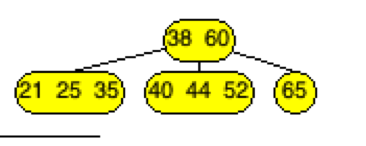
\includegraphics{pictures/tree30.png}
\caption{Imbalance in left subtree of right child}
\label{fig:tree30}
\end{figure}

The second set of images shows that key 52 has been moved to the root node, and key 60 has been moved to the right most child of the root to increase the size of that node.

\begin{figure}[H]
\centering
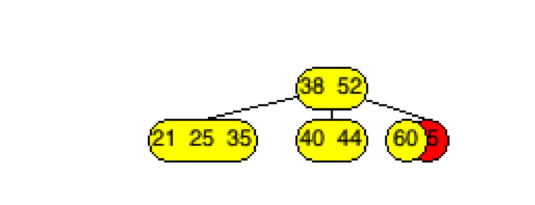
\includegraphics{pictures/tree31.png}
\caption{52 to parent. 60 to right node}
\label{fig:tree31}
\end{figure}

\begin{figure}[H]
\centering
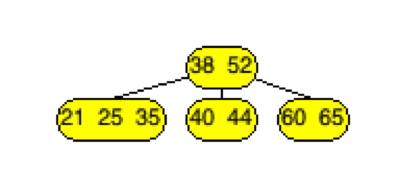
\includegraphics{pictures/tree32.png}
\caption{Balanced B-Tree}
\label{fig:tree32}
\end{figure}

The algorithms for insertion and removal into b-trees are straightforward but there are many cases required to accommodate resizing the nodes. The cases for insertion and deletion can be summarized as follows:
\begin{itemize}
	\item Inserting a key into a node within the min/max parameters
\begin{itemize}
	\item Key is simply inserted
\end{itemize}
	\item Inserting a key into a node that is full
\begin{itemize}
	\item Node is split into three (two children and a root)
	\item The root is given to the parent node
\begin{itemize}
	\item May result in the parent node being split
\end{itemize}
\end{itemize}
	\item Deleting a key from a leaf node that has at least 2 more than minimum
\begin{itemize}
	\item Key is simply deleted
\end{itemize}
	\item Deleting a key from a leaf node that has only 1 more than minimum
\begin{itemize}
	\item Key is deleted
	\item If a sibling node has an extra key, a rotation is done to move the extra key to the parent and a parent’s key to the underfull child
	\item If a sibling node does not have an extra key, nodes must be deleted and recombined
\end{itemize}
	\item Deleting a key from an internal node
\begin{itemize}
	\item Rotations must be performed to ensure that the keys in the internal node are greater than or equal to the keys in the appropriate subtree.
\end{itemize}
\end{itemize}

\section{Complexity}

\section{Summary}

After working through these materials you should be able to implement an AVL tree using a lazy delete strategy.  With a little bit of thinking you should be able to identify an algorithm for a direct delete for an AVL tree.  You should understand what a binary search tree is, and you should easily be able to read any online resource about the other types of binary search trees.  

 You should also understand the concepts behind b-trees and 2-3 trees (a specialized version of b-trees).   

\section{Additional Resources}
\begin{itemize}
	\item Mark Weiss, Data Structures and Algorithms in C++
	\item http://www.drdobbs.com/database/avl-trees/184404363
	\item http://www.bluerwhite.org/btree/
\end{itemize}

